\subsection{Conceptual Data Model}

This section introduces the abstract structure of how system information is conceptually organized. A conceptual data model translates business logic and system requirements into logical, technology-independent entities, enabling seamless integration with any database or platform \cite{larman-uml-patterns}. Accordingly, this section presents a conceptual representation of the application's data, including its validation rules and entity specifications.

\subsubsection{Conceptual Data Schema}

The system's conceptual data schema is presented in Figure \ref{fig:conceptual-data-schema}. It includes the main domain entities (classes), their essential properties (attributes), and the relationships among them (associations, aggregations, compositions, and generalizations).

\begin{figure}[H]
    \centering
    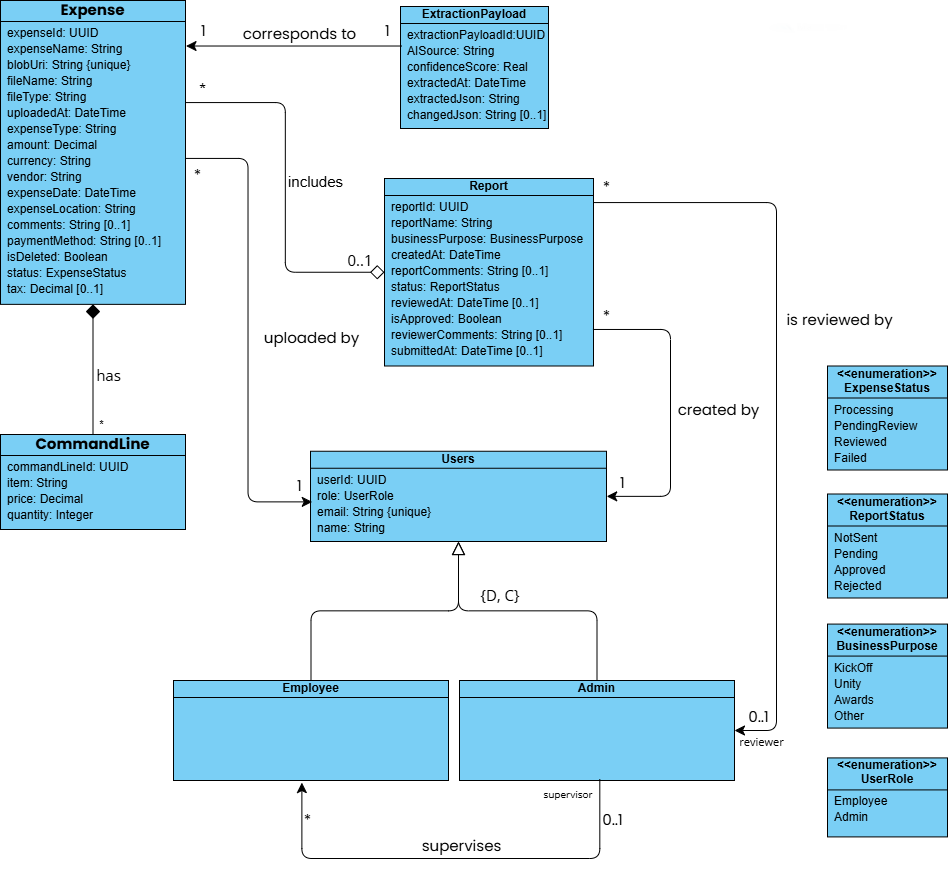
\includegraphics[width=\textwidth]{Images/UML.png}
    \caption[Conceptual data schema]
    {Conceptual data schema. [Own creation]}
    \label{fig:conceptual-data-schema}
\end{figure}

\newpage


\subsubsection{Integrity Constraints}

To ensure a valid and consistent data conceptual schema, the following integrity constraints must be applied:

\textbf{Primary keys:} (User, userId), (Expense, expenseId), (CommandLine, commandLineId), (ExtractionPayload, extractionPayloadId), (Report, reportId).

\textbf{RT2:} A user is classified as either an Employee or an Admin, depending on their assigned role.

\textbf{RT3:} An administrator can only review reports submitted by employees under their supervision.

\textbf{RT4:} The expense amount and tax must be greater than 0.

\textbf{RT5:} The expense currency must be a valid international currency.

\textbf{RT6:} The user's email must be a valid email address.

\textbf{RT7:} The expense date must be earlier than the current date.

\textbf{RT8:} The expenseDate timestamp must be earlier than the uploadedAt timestamp of the same expense.

\textbf{RT9:} The expense payment method must be either “cash” or “credit card”.

\textbf{RT10:} The command line price must be greater than or equal to 0.

\textbf{RT11:} The command line quantity must be greater than or equal to 1.

\textbf{RT12:} The extraction payload confidence score must be between 0 and 1.

\textbf{RT13:} The report submittedAt timestamp must not be null if the report status is “Pending”, “Approved”, or “Rejected”.

\textbf{RT14:} The report reviewedAt timestamp must not be null if the report status is “Approved” or “Rejected”.

\textbf{RT15:} The report's createdAt timestamp must be earlier than the submittedAt timestamp (if the latter is not null).

\textbf{RT16:} The report's submittedAt timestamp must be earlier than the reviewedAt timestamp (if both are not null).

\textbf{RT17:} An expense can be attached to a report only if the report is created by the same user who uploaded the expense.

\textbf{RT18:} A report status may transition from “NotSent” to “Submitted”, and from “Submitted” to “Approved” or “Rejected”.

\textbf{RT19:} A report without attached expenses is not allowed to transition to any status other than “NotSent”.

\subsubsection{Class Descriptions}

Each class in the conceptual data schema is described with a brief overview and a short description of its attributes.


\textbf{User}

This class represents the application's end users. Any individual who can log in to the application is considered a user. Each user is classified as either an Employee or an Admin. Consequently, users cannot review their own reports; administrators are only permitted to review reports submitted by employees under their supervision.

\begin{itemize} [leftmargin=0.75cm, noitemsep, label=\textbullet]

    \item \textbf{userId:} Unique identifier of the user. 
    
    \begin{itemize} [leftmargin=0.75cm, noitemsep, label=$\circ$]

        \item \textbf{type:} UUID.

        \item \textbf{constraints:} mandatory, unique, non-null.

    \end{itemize}

    \item \textbf{role:} Assigned role of the user.
    
    \begin{itemize} [leftmargin=0.75cm, noitemsep, label=$\circ$]

        \item \textbf{type:} UserRole Enum (Employee, Admin).

        \item \textbf{constraints:} mandatory, non-null.

    \end{itemize}

    \item \textbf{email:} Corporate email address of the user, used for authentication.
    
    \begin{itemize} [leftmargin=0.75cm, noitemsep, label=$\circ$]

        \item \textbf{type:} String.

        \item \textbf{constraints:} mandatory, unique, must follow a valid email format.

    \end{itemize}

    \item \textbf{name:} Full name of the user.
    
    \begin{itemize} [leftmargin=0.75cm, noitemsep, label=$\circ$]

        \item \textbf{type:} String.

        \item \textbf{constraints:} mandatory, non-null
        
    \end{itemize}

\end{itemize}
\textbf{Expense}

This class represents an expense submitted by a user. Each expense must be associated with the user who uploaded it.

\begin{itemize} [leftmargin=0.75cm, noitemsep, label=\textbullet]

    \item \textbf{expenseId:} Unique identifier of the expense.
    
    \begin{itemize} [leftmargin=0.75cm, noitemsep, label=$\circ$]

        \item \textbf{type:} UUID.

        \item \textbf{constraints:} mandatory, unique, non-null.

    \end{itemize}

    \item \textbf{expenseName:} Name assigned to the expense by the user.
    
    \begin{itemize} [leftmargin=0.75cm, noitemsep, label=$\circ$]

        \item \textbf{type:} String.

        \item \textbf{constraints:} mandatory, non-null.

    \end{itemize}

    \item \textbf{blobUri:} URI of the stored expense file.
    
    \begin{itemize} [leftmargin=0.75cm, noitemsep, label=$\circ$]

        \item \textbf{type:} String.

        \item \textbf{constraints:} mandatory, unique, non-null.

    \end{itemize}

    \item \textbf{fileName:} Name of the uploaded file.
    
    \begin{itemize} [leftmargin=0.75cm, noitemsep, label=$\circ$]

        \item \textbf{type:} String.

        \item \textbf{constraints:} mandatory, non-null.

    \end{itemize}

    \item \textbf{fileType:} Type of the uploaded file (e.g., PDF, JPEG).
    
    \begin{itemize} [leftmargin=0.75cm, noitemsep, label=$\circ$]

        \item \textbf{type:} String.

        \item \textbf{constraints:} mandatory, non-null.

    \end{itemize}

    \item \textbf{uploadedAt:} Timestamp indicating when the expense was uploaded.
    
    \begin{itemize} [leftmargin=0.75cm, noitemsep, label=$\circ$]

        \item \textbf{type:} DateTime.

        \item \textbf{constraints:} mandatory, non-null.

    \end{itemize}

    \item \textbf{expenseType:} Category of the expense (e.g., travel, meals).
    
    \begin{itemize} [leftmargin=0.75cm, noitemsep, label=$\circ$]

        \item \textbf{type:} String.

        \item \textbf{constraints:} mandatory, non-null.

    \end{itemize}

    \item \textbf{amount:} Monetary amount of the expense.
    
    \begin{itemize} [leftmargin=0.75cm, noitemsep, label=$\circ$]

        \item \textbf{type:} Decimal.

        \item \textbf{constraints:} mandatory, non-null, must be $\geq 0$.

    \end{itemize}

    \item \textbf{currency:} Currency of the expense amount (e.g., EUR, USD).
    
    \begin{itemize} [leftmargin=0.75cm, noitemsep, label=$\circ$]

        \item \textbf{type:} String.

        \item \textbf{constraints:} mandatory, non-null, must be a valid international currency code.

    \end{itemize}

    \item \textbf{vendor:} Name of the vendor or service provider.
    
    \begin{itemize} [leftmargin=0.75cm, noitemsep, label=$\circ$]

        \item \textbf{type:} String.

        \item \textbf{constraints:} mandatory, non-null.

    \end{itemize}

    \item \textbf{expenseDate:} Date when the expense was incurred.
    
    \begin{itemize} [leftmargin=0.75cm, noitemsep, label=$\circ$]

        \item \textbf{type:} DateTime.

        \item \textbf{constraints:} mandatory, non-null, must be $\leq$ current datetime and uploaded datetime.

    \end{itemize}

    \item \textbf{expenseLocation:} Location where the expense was incurred.
    
    \begin{itemize} [leftmargin=0.75cm, noitemsep, label=$\circ$]

        \item \textbf{type:} String.

        \item \textbf{constraints:} mandatory, non-null.

    \end{itemize}

    \item \textbf{comments:} Additional notes or description provided by the user.
    
    \begin{itemize} [leftmargin=0.75cm, noitemsep, label=$\circ$]

        \item \textbf{type:} String.

        \item \textbf{constraints:} optional.

    \end{itemize}

    \item \textbf{paymentMethod:} Method used for the payment (e.g., cash, credit card).
    
    \begin{itemize} [leftmargin=0.75cm, noitemsep, label=$\circ$]

        \item \textbf{type:} String.

        \item \textbf{constraints:} optional.

    \end{itemize}

    \item \textbf{isDeleted:} Indicates whether the expense has been logically deleted.
    
    \begin{itemize} [leftmargin=0.75cm, noitemsep, label=$\circ$]

        \item \textbf{type:} Boolean.

        \item \textbf{constraints:} mandatory, default = false.

    \end{itemize} 

    \item \textbf{status:} Current AI extraction process status of the expense.
    
    \begin{itemize} [leftmargin=0.75cm, noitemsep, label=$\circ$]

        \item \textbf{type:} ExpenseStatus Enum (Processing, PendingReview, Reviewed, Failed).

        \item \textbf{constraints:} mandatory, non-null.

    \end{itemize}

    \item \textbf{tax:} Tax amount associated with the expense.
    
    \begin{itemize} [leftmargin=0.75cm, noitemsep, label=$\circ$]

        \item \textbf{type:} Decimal.

        \item \textbf{constraints:} optional, must be $\geq 0$.

    \end{itemize}

\end{itemize}
\textbf{CommandLine}

This class represents an individual line item within an expense, typically corresponding to a specific product or service listed on a receipt. If the associated expense is deleted, the command line must also be deleted.

\begin{itemize} [leftmargin=0.75cm, noitemsep, label=\textbullet]

    \item \textbf{commandLineId:} Unique identifier of the command line.
    
    \begin{itemize} [leftmargin=0.75cm, noitemsep, label=$\circ$]

        \item \textbf{type:} UUID.

        \item \textbf{constraints:} mandatory, unique, non-null.

    \end{itemize}

    \item \textbf{item:} Description or name of the purchased item or service.
    
    \begin{itemize} [leftmargin=0.75cm, noitemsep, label=$\circ$]

        \item \textbf{type:} String.

        \item \textbf{constraints:} mandatory, non-null.

    \end{itemize}

    \newpage

    \item \textbf{quantity:} Number of units of the item.
    
    \begin{itemize} [leftmargin=0.75cm, noitemsep, label=$\circ$]

        \item \textbf{type:} Integer.

        \item \textbf{constraints:} mandatory, non-null, must be $\geq 1$.

    \end{itemize}

    \item \textbf{price:} Monetary value of the item.
    
    \begin{itemize} [leftmargin=0.75cm, noitemsep, label=$\circ$]

        \item \textbf{type:} Decimal.

        \item \textbf{constraints:} mandatory, non-null, must be $\geq 0$.

    \end{itemize}

\end{itemize}
\textbf{ExtractionPayload}

This class represents the data extracted from an expense using an AI service. An extraction Payload must always correspond to a single, unique expense.

\begin{itemize} [leftmargin=0.75cm, noitemsep, label=\textbullet]

    \item \textbf{extractionPayloadId:} Unique identifier of the extraction payload.
    
    \begin{itemize} [leftmargin=0.75cm, noitemsep, label=$\circ$]

        \item \textbf{type:} UUID.

        \item \textbf{constraints:} mandatory, unique, non-null.

    \end{itemize}

    \item \textbf{aiSource:} Identifier of the AI service or model used for extraction.
    
    \begin{itemize} [leftmargin=0.75cm, noitemsep, label=$\circ$]

        \item \textbf{type:} String.

        \item \textbf{constraints:} mandatory, non-null.

    \end{itemize}

    \item \textbf{confidenceScore:} Confidence level assigned by the AI to the extracted data.
    
    \begin{itemize} [leftmargin=0.75cm, noitemsep, label=$\circ$]

        \item \textbf{type:} Real.

        \item \textbf{constraints:} mandatory, non-null, must be between 0 and 1.

    \end{itemize}

    \item \textbf{extractedAt:} Timestamp indicating when the data was extracted.
    
    \begin{itemize} [leftmargin=0.75cm, noitemsep, label=$\circ$]

        \item \textbf{type:} DateTime.

        \item \textbf{constraints:} mandatory, non-null.

    \end{itemize}

    \item \textbf{extractedJson:} Raw data extracted by the AI in JSON format.
    
    \begin{itemize} [leftmargin=0.75cm, noitemsep, label=$\circ$]

        \item \textbf{type:} String.

        \item \textbf{constraints:} mandatory, non-null.

    \end{itemize}

    \item \textbf{changedJson:} Modified version of the extracted data after user adjustments.
    
    \begin{itemize} [leftmargin=0.75cm, noitemsep, label=$\circ$]

        \item \textbf{type:} String.

        \item \textbf{constraints:} optional.

    \end{itemize}

\end{itemize}
\textbf{Report}

This class represents a collection of expenses grouped together for submission and review. A report must always belong to the user who created it, and it can only be reviewed by that user's supervisor.

\begin{itemize} [leftmargin=0.75cm, noitemsep, label=\textbullet]

    \item \textbf{reportId:} Unique identifier of the report.
    
    \begin{itemize} [leftmargin=0.75cm, noitemsep, label=$\circ$]

        \item \textbf{type:} UUID.

        \item \textbf{constraints:} mandatory, unique, non-null.

    \end{itemize}

    \item \textbf{reportName:} Name assigned to the report.
    
    \begin{itemize} [leftmargin=0.75cm, noitemsep, label=$\circ$]

        \item \textbf{type:} String.

        \item \textbf{constraints:} mandatory, non-null.

    \end{itemize}

    \item \textbf{businessPurpose:} Business purpose of the report.
    
    \begin{itemize} [leftmargin=0.75cm, noitemsep, label=$\circ$]

        \item \textbf{type:} BusinessPurpose Enum (KickOff, Unity, Awards, Other).

        \item \textbf{constraints:} mandatory, non-null.

    \end{itemize}

    \newpage

    \item \textbf{createdAt:} Timestamp indicating when the report was created.
    
    \begin{itemize} [leftmargin=0.75cm, noitemsep, label=$\circ$]

        \item \textbf{type:} DateTime.

        \item \textbf{constraints:} mandatory, non-null.

    \end{itemize}

    \item \textbf{reportComments:} Additional comments or notes provided by the user.
    
    \begin{itemize} [leftmargin=0.75cm, noitemsep, label=$\circ$]

        \item \textbf{type:} String.

        \item \textbf{constraints:} optional.

    \end{itemize}

    \item \textbf{status:} Current status of the report.
    
    \begin{itemize} [leftmargin=0.75cm, noitemsep, label=$\circ$]

        \item \textbf{type:} ReportStatus Enum (NotSent, Pending, Approved, Rejected).

        \item \textbf{constraints:} mandatory, non-null.

    \end{itemize}

    \item \textbf{submittedAt:} Timestamp indicating when the report was submitted.
    
    \begin{itemize} [leftmargin=0.75cm, noitemsep, label=$\circ$]

        \item \textbf{type:} DateTime.

        \item \textbf{constraints:} optional (null if not yet submitted).

    \end{itemize}

    \item \textbf{reviewedAt:} Timestamp indicating when the report was reviewed.
    
    \begin{itemize} [leftmargin=0.75cm, noitemsep, label=$\circ$]

        \item \textbf{type:} DateTime.

        \item \textbf{constraints:} optional (null if not yet reviewed).

    \end{itemize}

    \item \textbf{isApproved:} Indicates whether the report has been approved.
    
    \begin{itemize} [leftmargin=0.75cm, noitemsep, label=$\circ$]

        \item \textbf{type:} Boolean.

        \item \textbf{constraints:} mandatory, default = false.

    \end{itemize}

    \item \textbf{reviewerComments:} Comments provided by the reviewer during the review process.
    
    \begin{itemize} [leftmargin=0.75cm, noitemsep, label=$\circ$]

        \item \textbf{type:} String.

        \item \textbf{constraints:} optional.

    \end{itemize}

\end{itemize}

